\documentclass{standalone}

\usepackage{tikz}
\usepackage{tkz-euclide}
\usetikzlibrary{calc}
\usetikzlibrary{positioning}
\usetikzlibrary{arrows.meta}

\usepackage{times}


\begin{document}
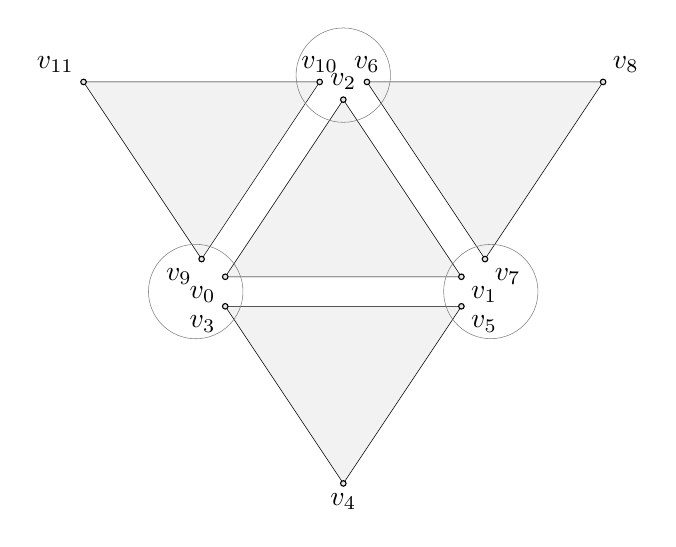
\begin{tikzpicture}[%
  >={Stealth[scale=1.0]},
  scale=1.5,
]

  \tkzDefPoint(0.0, 0.0){v0}
  \tkzDefPoint(2.0, 0.0){v1}
  \tkzDefPoint(1.0, 1.5){v2}

  \tkzDefPoint(0.0, -0.25){v3}
  \tkzDefPoint(1.0, -1.75){v4}
  \tkzDefPoint(2.0, -0.25){v5}

  \tkzDefPoint(1.2, 1.65){v6}
  \tkzDefPoint(2.2, 0.15){v7}
  \tkzDefPoint(3.2, 1.65){v8}

  \tkzDefPoint(-0.2, 0.15){v9}
  \tkzDefPoint(0.8, 1.65){v10}
  \tkzDefPoint(-1.2, 1.65){v11}

  \tkzDrawPolygon[fill=black!5](v0,v1,v2)
  \tkzDrawPolygon[fill=black!5](v3,v4,v5)
  \tkzDrawPolygon[fill=black!5](v6,v7,v8)
  \tkzDrawPolygon[fill=black!5](v9,v10,v11)

  \tkzDefTriangleCenter[circum](v0,v3,v9)\tkzGetPoint{A}
  \tkzDefCircle[R](A,0.4)\tkzGetPoint{AR}
  \tkzDrawCircle(A,AR)

  \tkzDefTriangleCenter[circum](v1,v5,v7)\tkzGetPoint{B}
  \tkzDefCircle[R](B,0.4)\tkzGetPoint{BR}
  \tkzDrawCircle(B,BR)

  \tkzDefTriangleCenter[circum](v2,v6,v10)\tkzGetPoint{C}
  \tkzDefCircle[R](C,0.4)\tkzGetPoint{CR}
  \tkzDrawCircle(C,CR)

  \tkzDrawPoints(v0,v1,v2,v3,v4,v5,v6,v7,v8,v9,v10,v11)

  \tkzLabelPoint[below left](v0){$v_0$}
  \tkzLabelPoint[below right](v1){$v_1$}
  \tkzLabelPoint[above](v2){$v_2$}

  \tkzLabelPoint[below left](v3){$v_3$}
  \tkzLabelPoint[below](v4){$v_4$}
  \tkzLabelPoint[below right](v5){$v_5$}

  \tkzLabelPoint[above](v6){$v_6$}
  \tkzLabelPoint[below right](v7){$v_7$}
  \tkzLabelPoint[above right](v8){$v_8$}

  \tkzLabelPoint[below left](v9){$v_9$}
  \tkzLabelPoint[above](v10){$v_{10}$}
  \tkzLabelPoint[above left](v11){$v_{11}$}

\end{tikzpicture}
\end{document}
